\documentclass[rebuttal]{cvpr}

\usepackage{times}
\usepackage{epsfig}
\usepackage{graphicx}
\usepackage{graphics}
\usepackage{amsmath}
\usepackage{amssymb}
\usepackage{listings}

% Include other packages here, before hyperref.
\usepackage{multirow, multicol, booktabs}
\usepackage{caption}
\usepackage{subcaption}
\usepackage{tabularx}

\newcommand{\todoc}[2]{{\textcolor{#1} {\textbf{[#2]}}}}
\newcommand{\todored}[1]{\todoc{red}{\textbf{#1}}}
\newcommand{\TA}[1]{\todored{TA: #1}}

% Include other packages here, before hyperref.

% If you comment hyperref and then uncomment it, you should delete
% egpaper.aux before re-running latex.  (Or just hit 'q' on the first latex
% run, let it finish, and you should be clear).
\usepackage[pagebackref=true,breaklinks=true,colorlinks,bookmarks=false]{hyperref}
%%%%%%%%% PAPER ID  - PLEASE UPDATE
\def\cvprPaperID{0000} % Do not enter team number here
%\def\httilde{\mbox{\tt\raisebox{-.5ex}{\symbol{126}}}}

\def\cvprPaperID{0000} % Do not enter team number here
\def\confYear{AI604 2021 spring}

\begin{document}

%%%%%%%%% TITLE - PLEASE UPDATE
\title{AI604 term project rebuttal / author response}  % **** Enter the paper title here

\maketitle
\thispagestyle{empty}


%%%%%%%%% BODY TEXT - ENTER YOUR RESPONSE BELOW
% \section{Introduction}

% After receiving paper reviews, authors should submit a rebuttal to address the reviewers' comments, which will be limited to a {\bf one page} PDF file.

% Note that the author rebuttal is not visible to the reviewers. In other words, only TAs and the professor will read the rebuttal. 

% \subsection{Response length}

% Author responses must be no longer than 1 page in length except for \textbf{References} and \textbf{Additional question}.

% \subsection{Note}

% Feel free to write the author response, and we recommend you not to spend your time so much on this. We aim to provide you a chance to improve your work by answering to the reviews. Each team will receive five or six reviews. 

% \TA{Remove guidelines (Section 1) and write your response.}

%-------------------------------------------------------------------------
%\newpage

\section{Additional question}
% Each team should answer the below questions for evaluating their reviewers.

\subsection{Question 1}
\begin{itemize}
    % 리뷰어 1 2 3 4 5 6 은 우리의 프로젝트 내용을 이해했다.
    \item The reviewer 1 understood our main idea and contributions. \textbf{Yes}
    
    \item The reviewer 2 understood our main idea and contributions. \textbf{Yes}
    
    \item The reviewer 3 understood our main idea and contributions. \textbf{Yes}
    
    \item The reviewer 4 understood our main idea and contributions. \textbf{Yes}
    \item The reviewer 5 understood our main idea and contributions. \textbf{Yes}
    
    \item The reviewer 6 understood our main idea and contributions. \textbf{Yes}
\end{itemize}

\subsection{Question 2}
\begin{itemize}
    % 리뷰어 1 2 3 4 5 6 은 우리에게 건설적인 피드백을 제공했다.
    \item The reviewer 1 provided constructive feedback or advice. \textbf{No}, no suggestion was given.
    
    \item The reviewer 2 provided constructive feedback or advice.
    \textbf{No}, no suggestion was given.
    
    \item The reviewer 3 provided constructive feedback or advice. \textbf{Yes}, we will include computation costs and GPU memory comparison experiments in our following reports. The reviewer also suggested including Transformer architecture diagram, but we shall decide according to the length of the final version of the paper. We made changes to the diagrams to make it clearer (Figure \ref{fig:seg+class} \ref{fig:class} \ref{fig:seg} ). We will be providing better explanations for the training procedure in the upcoming versions.
    
    \item The reviewer 4 provided constructive feedback or advice. \textbf{Yes}, the explanations on how the segmentation reconstruction head works will be provided in the later versions. Our approach will be mostly convolution-free (mathematical operation-wise), and we are still investigating various methods for reconstruction. The experiment setup will be further organized and released accordingly. Note that the experiments provided in the progress report were only preliminary, and more experiments may be conducted with different settings.
    
    \item The reviewer 5 provided constructive feedback or advice. \textbf{Yes}, the reviewer asked some questions. For the first question, pixel-by-pixel accuracy is sometimes used as evaluation metric in segmentation tasks. It is often provided as 
    \[ \text{Acc} := \frac{TP + TN}{TP + TN + FP + FN} \]
    However, intersection-over-union (IoU) or other metrics designed for segmentation are often preferred because pixel-by-pixel accuracy can provide misleading results when the class representation is small within the image. This is because the measure can be biased in reporting how well the model identify non-present class. In our particular dataset, there are some small regions in the image, which can lead to misleading metrics. 
    
    For the second question, domain adaptation and transfer learning are often used interchangeably in computer vision literature. Even though it is not entirely correct, but we follow through with the general academic consensus. In our case with medical image tasks, domain adaptation can be helpful in a case where the model needs to be adopted in different hospitals. The model is expected to perform equally well with semantically similar but distributional different images, which is often the case in real-life circumstances.  
    
    \item The reviewer 6 provided constructive feedback or advice. \textbf{Neutral}. The author suggests some different variants of ViT such as DeiT and CaiT. Some of these model setups are already being investigated for the upcoming progress report. The author also says a large private dataset is needed for training ViT, but we have already observed nice performance in some of the preliminary experiments with both pretrained and non-pretrained models. We also plan to experiment with the recently proposed MLP Mixer, convolution- and attention-free model for images. 
\end{itemize}

\subsection{Question 3}
Redrawn figures in response to Reviewer 3 are provided below:

    \begin{figure}[ht]
    \begin{center}
       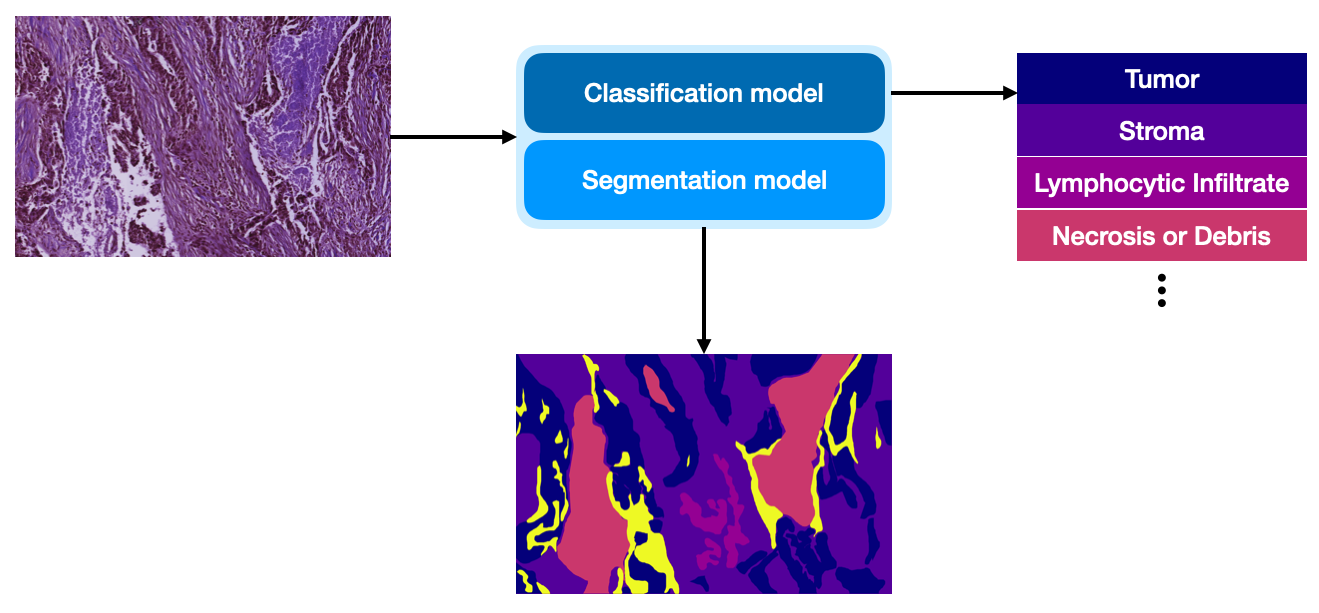
\includegraphics[width=0.8\linewidth]{media/Blockdiagram.png}
    \end{center}
       \caption{Block diagram of the model for WSIs segmentation and classification}
    \label{fig:seg+class}
    \end{figure}
    
    \begin{figure}[ht]
    \begin{center}
       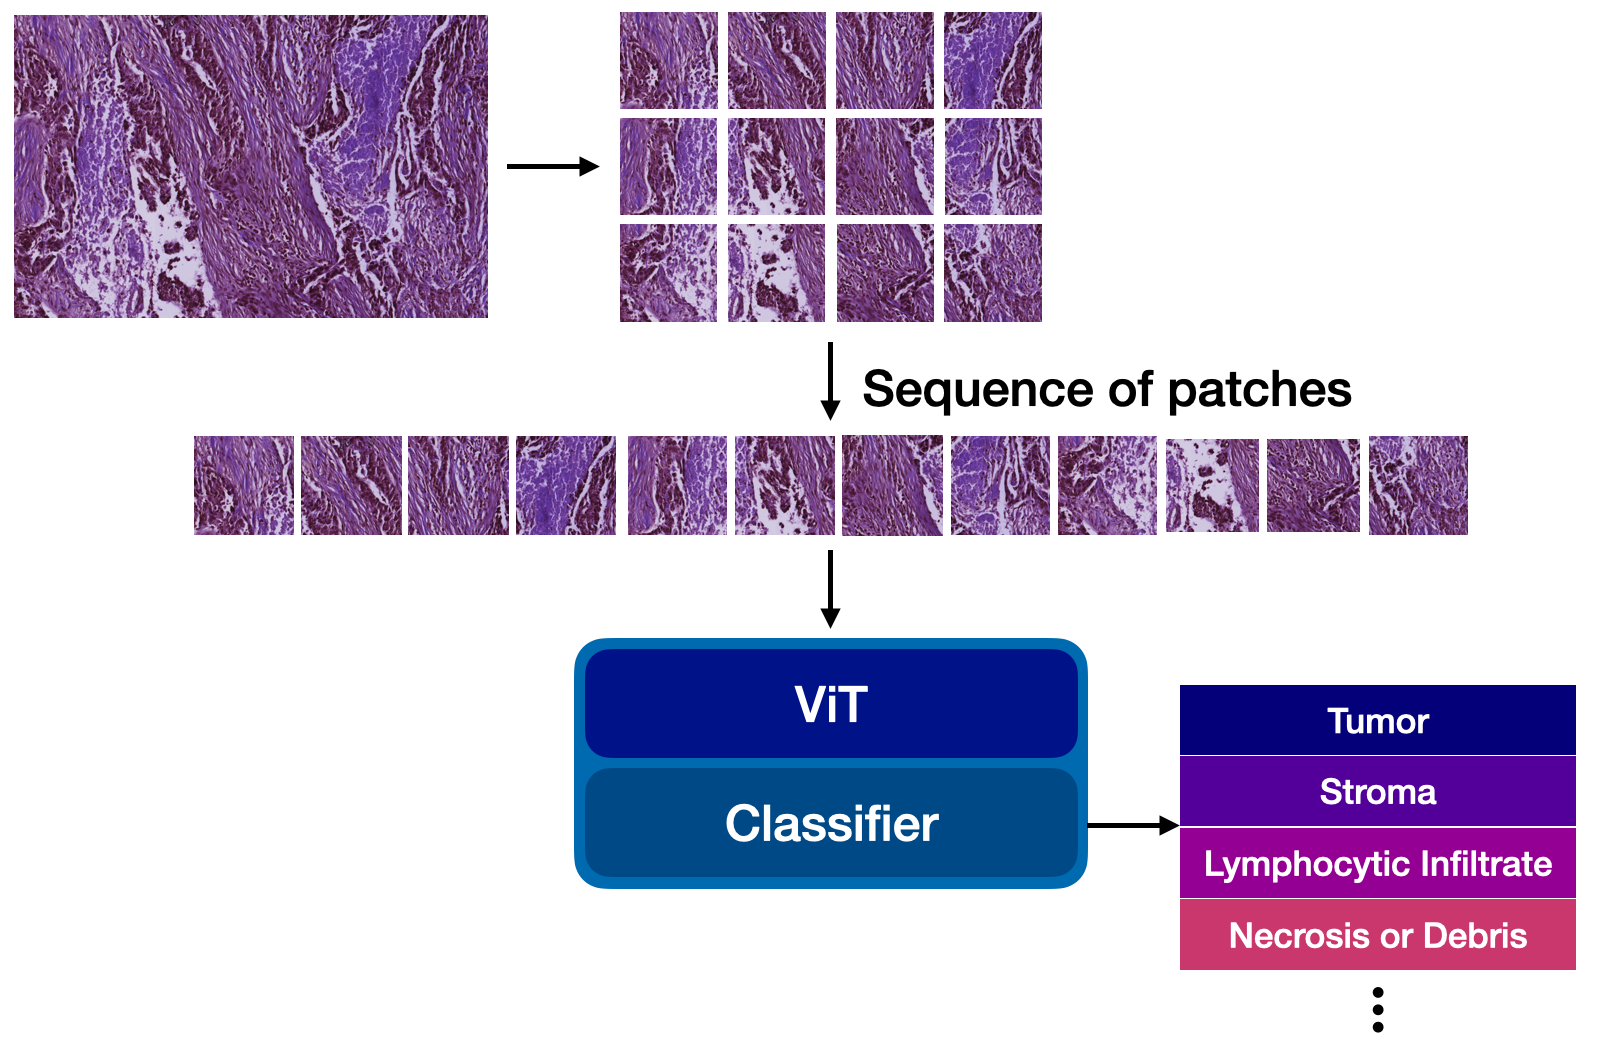
\includegraphics[width=0.8\linewidth]{media/classifier.png}
    \end{center}
       \caption{Block diagram of the model for WSIs classification}
    \label{fig:class}
    \end{figure}
    
    \begin{figure}[ht]
        \begin{subfigure}{0.5\textwidth}
            \centering
            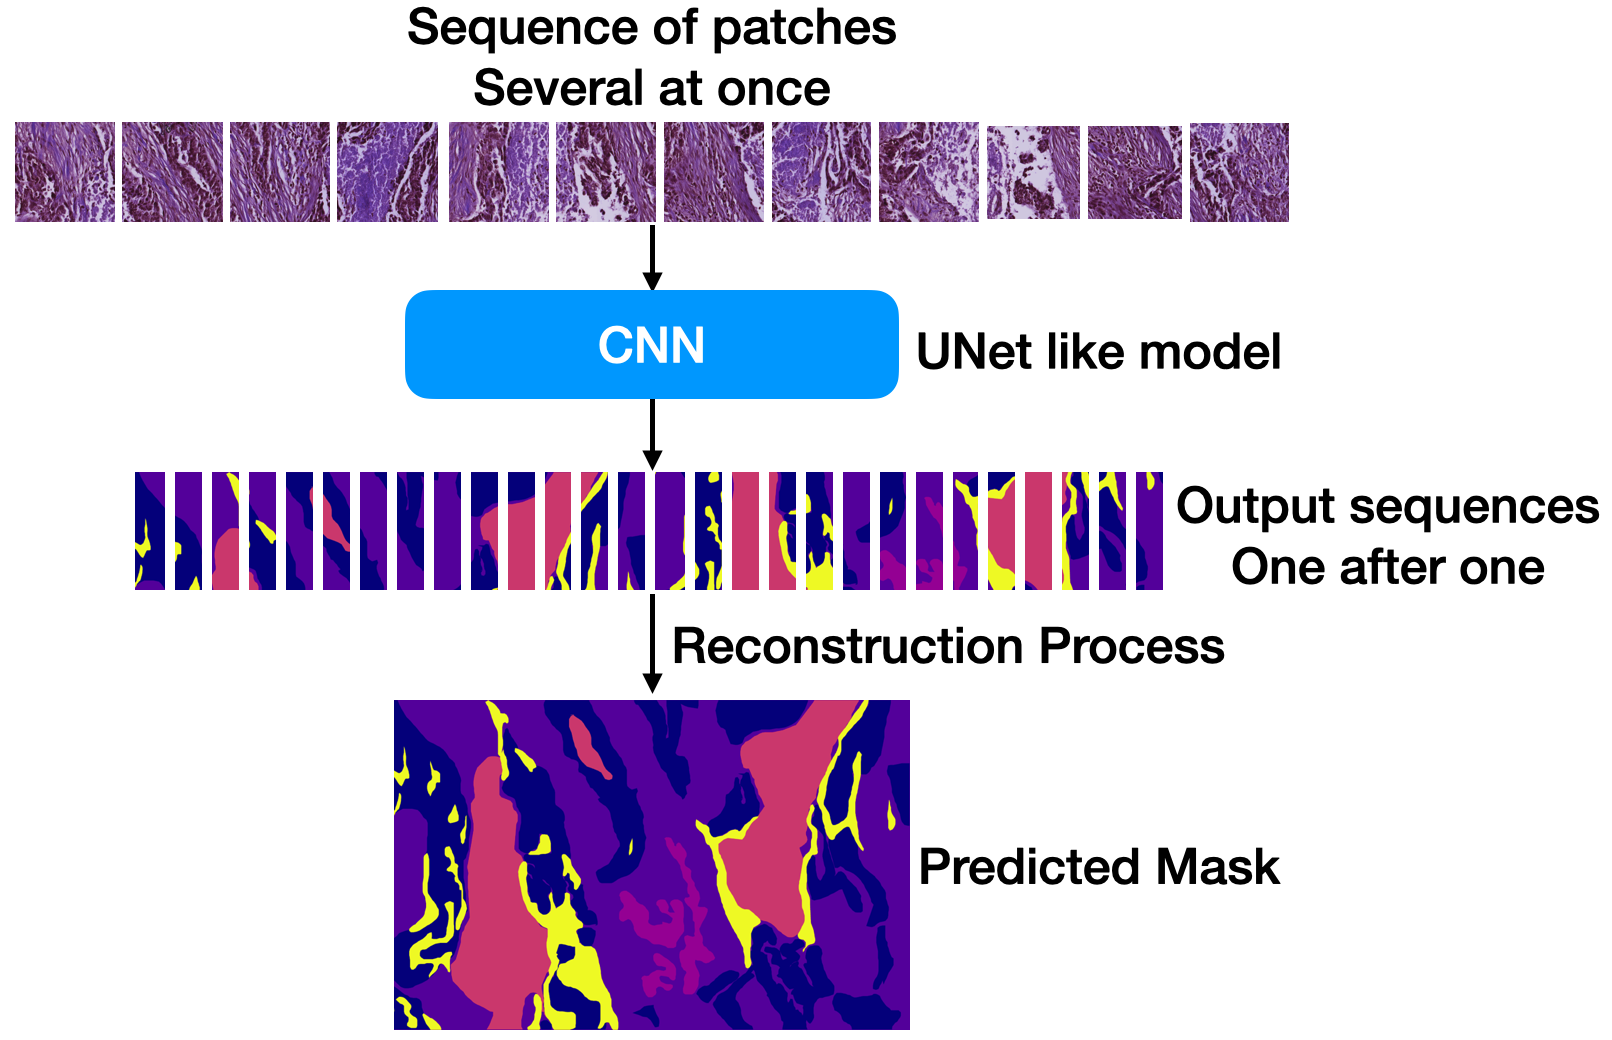
\includegraphics[width=0.8\linewidth]{media/previous-patch-based-approach.png}
            \caption{Previous patch-based approach}
            \label{fig:prev}
        \end{subfigure}
        \begin{subfigure}{0.5\textwidth}
            \centering
            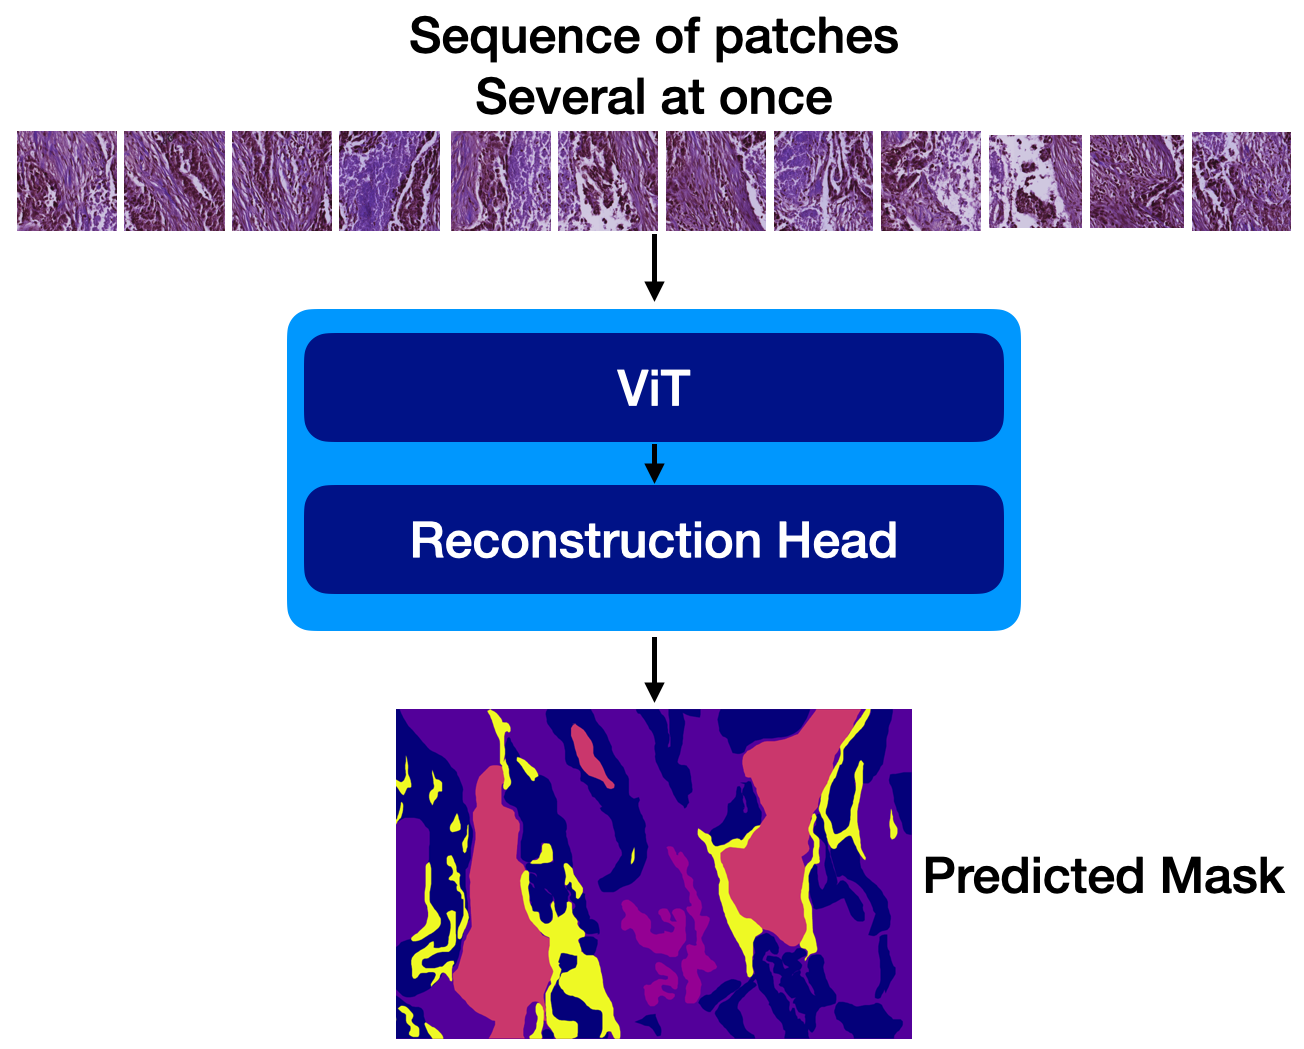
\includegraphics[width=0.8\linewidth]{media/proposed-seg.png}
            \caption{Proposed segmentation architecture}
            \label{fig:prop}
        \end{subfigure}
        \caption{WSI segmentation model diagram}
        \label{fig:seg}
    \end{figure}

% {\small
% \bibliographystyle{ieee_fullname}
% \bibliography{reference}
% }

\end{document}
